\chapter{Installing BeagleSNES}

\section{Overview}\index{Overview}

BeagleSNES is more than just a single application.  It is a complete POSIX operating system environment, complete with a custom Linux kernel, a full file system, and configuration files that tell BeagleSNES how to behave for the end user.  Because of the general complexity of such a large system, it can sometimes be difficult to get everything up and running smoothly.  This section will tell you how to download and install BeagleSNES so that you can get started using it as quickly and painlessly as possible.  

\begin{figure}[h]
\centering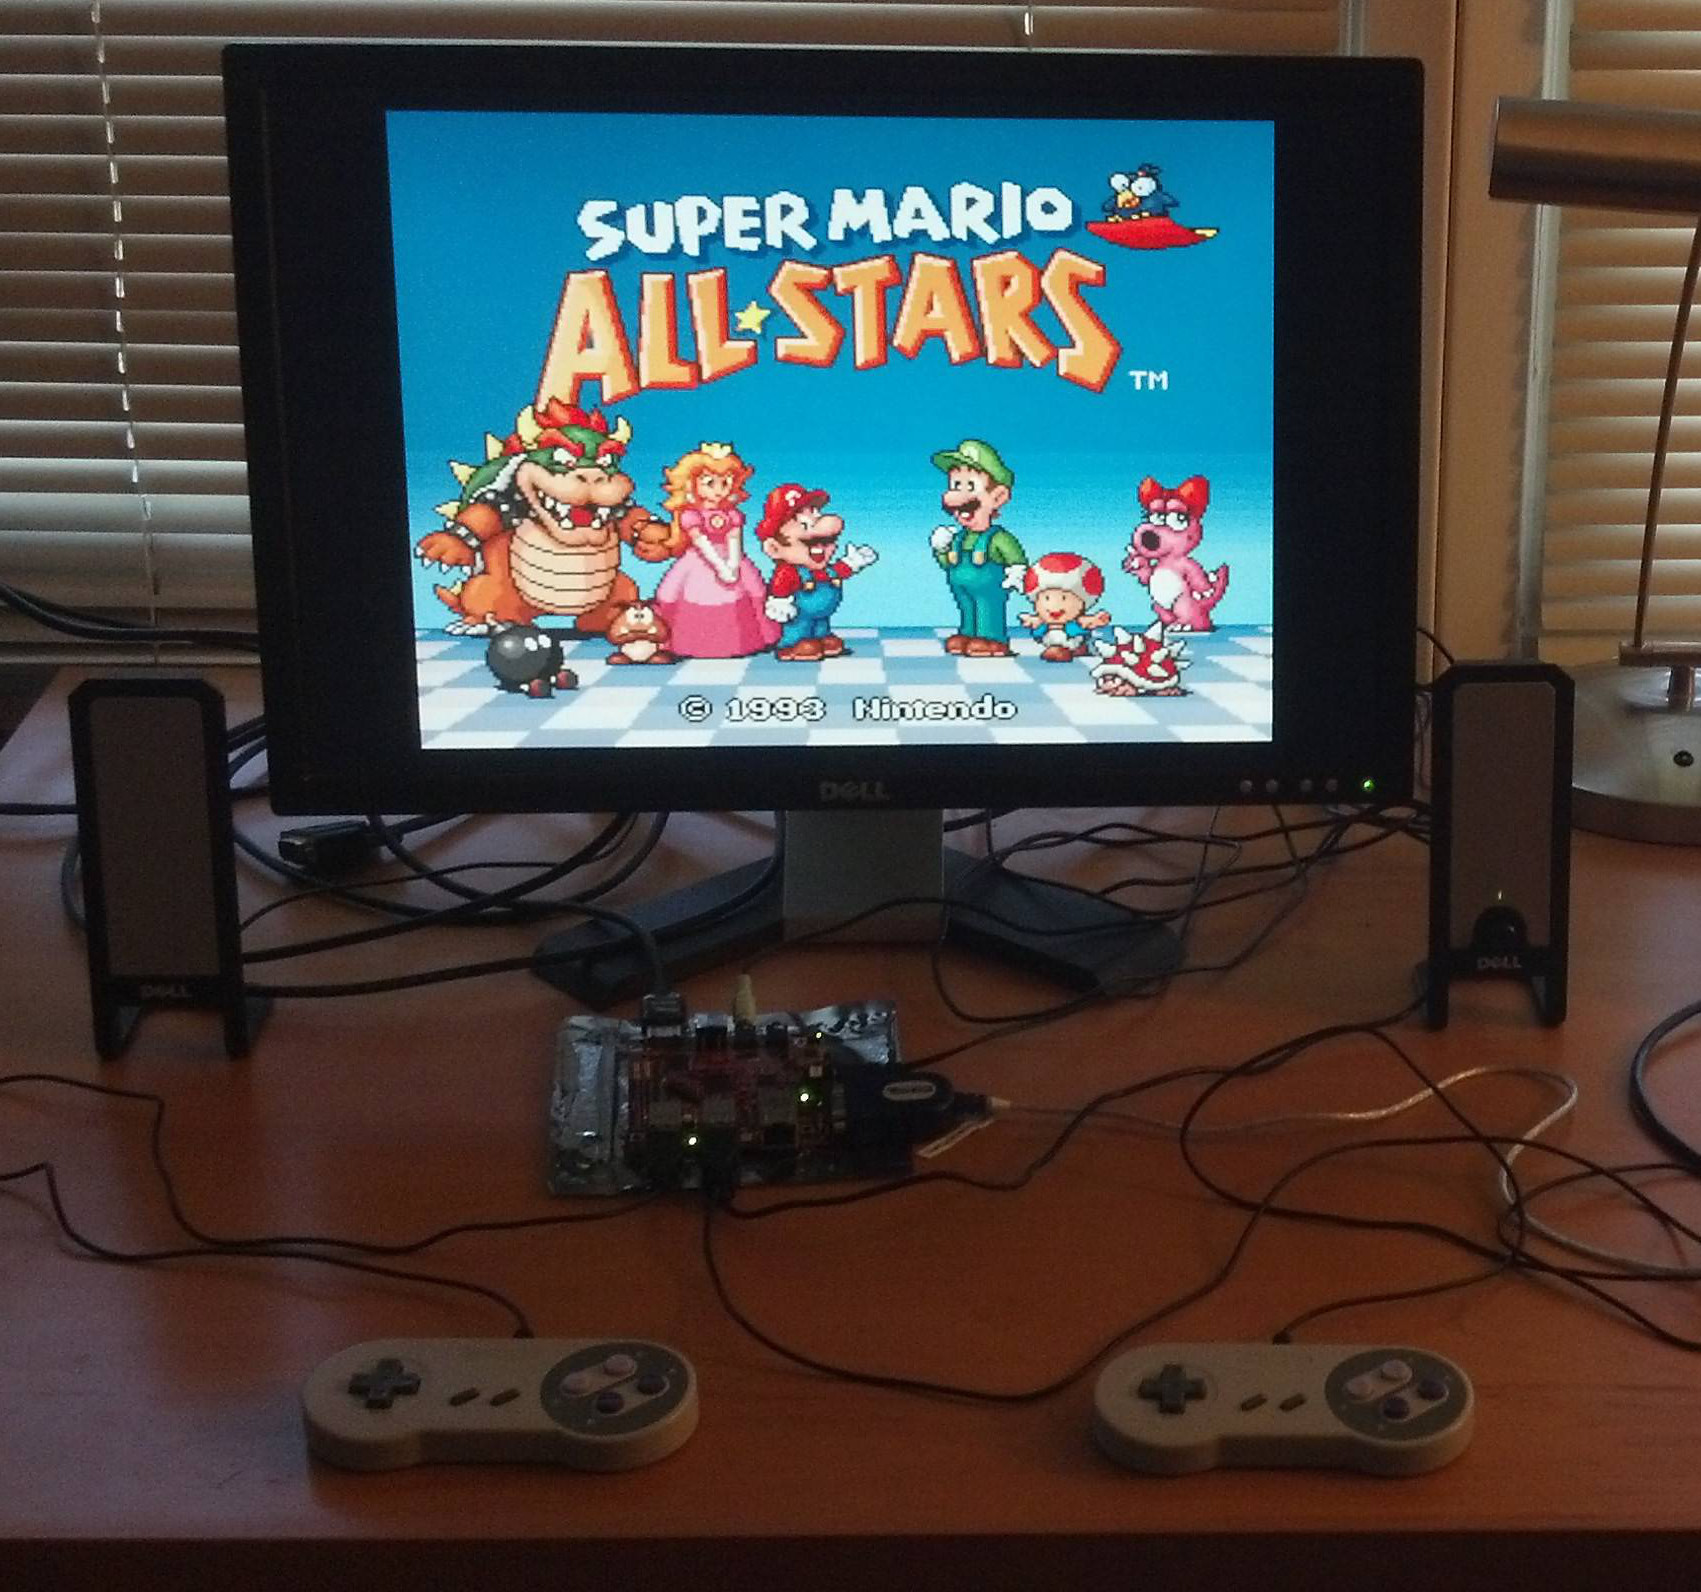
\includegraphics[scale=0.10,clip=true,trim=0 40 0 0]{install_chapter/BBxM_version.jpg}
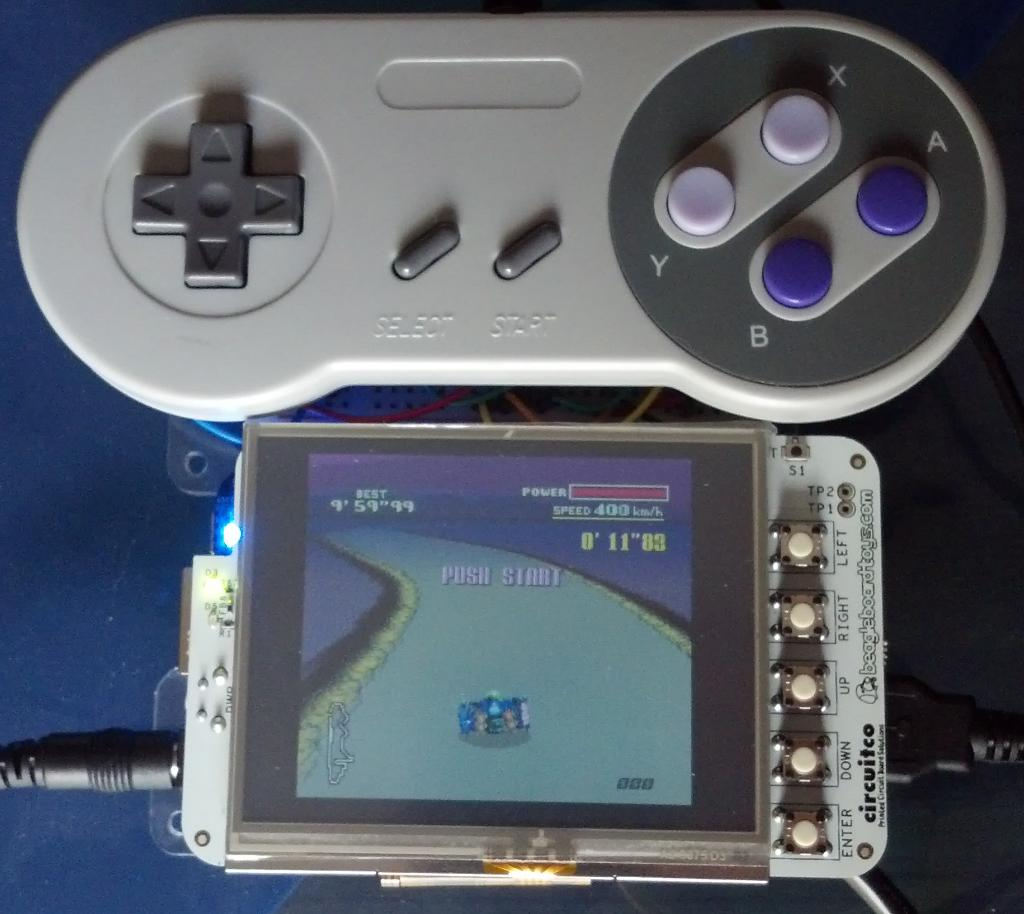
\includegraphics[scale=0.17]{install_chapter/LCD3_version.jpg}
\caption{The 0.5 release of BeagleSNES, running on the BB-xM with DVI digital video output (left) and on the BBB with the LCD3 cape (right).}
\end{figure}

All source code for the project, as well as a full file system image of a complete BeagleSNES system, have been made available for download.  Most users will only wish to try out BeagleSNES, rather than hack on its source code, so this section will focus on using the full file system image.  Prior to starting, you'll need the following items:

\begin{itemize}
\item Either a BB-xM hardware platform that is at least revision C or a BBB platform that is at least revision A5A.  Earlier revisions have not been tested and are not suggested.
\item An external power supply to provide full power to the system.  Powering via USB will not provide the necessary amount of current.
\item An HDMI-to-DVI cable (BB-xM) or microHDMI-to-HDMI cable (BBB), and a television or monitor capable of displaying the digital video signal.  Or, if you may wish to instead use a Circuitco LCD3 cape board for displaying video for the BBB.
\item For the BB-xM, external speakers or a headset for listening to the audio output\footnote{Even when using an HDMI-to-HDMI cable for the video, audio will not be transmitted over the cable.  This is because the signal being transmitted over the HDMI cable is actually a DVI signal (video only), rather than an HDMI signal that contains both video and audio data.}.  The audio for the BBB is sent over the HDMI connection. 
\item A microSD card with a capacity of at least 4 GB.  BeagleSNES will rewrite the partition table on this card, so make sure that it does not contain any data that you need.
\item Copies of the software ROMs that you wish to use with BeagleSNES.
\item One or two Tomee\texttrademark USB SNES Gamepad controller(s)\footnote{Several online vendors offer this particular USB controller for sale. It is the only controller that will be officially supported for BeagleSNES.}. The BB-xM supports using one or two controllers, but the BBB only supports one unless you use an external USB hub to provide additional USB ports.  \emph{USB controllers other than the Tomee\texttrademark will work with BeagleSNES}, but they will most likely need their buttons remapped.
\end{itemize}

\begin{updateWarn}
While many SNES ROMs are widely available on the web, possession of these ROMs is generally considered to be piracy of commercial software. No ROMs are provided in the BeagleSNES file system images, and no help in obtaining ROMs will be given.  You're on your own.
\end{updateWarn}

\section{Downloading}\index{Downloading}

There are two BeagleSNES file system images available for download. The first is a microSD card image that contains a complete BeagleSNES system (bootloader, kernel, file system, etc.).  The second is a tarball of only the directory structure that includes the BeagleSNES application, its associated resources, and sample configuration files.  This image is intended for more advanced users that wish to add the BeagleSNES emulator into an existing file system environment that they have created.  The complete microSD card image will be referred to as the \emph{full system image}, and the tarball of the BeagleSNES directory structure will be referred to as the \emph{application image}.  The contents of the application image already exist inside of the full system image.

Direct download links to the latest versions of all BeagleSNES software components are available at \texttt{www.beaglesnes.org}.  SourceForge hosts all of the files for BeagleSNES\footnote{\texttt{https://sourceforge.net/projects/beaglesnes/files/}}, but \texttt{www.beaglesnes.org} should first be consulted for any additional information that you might need about the latest version of BeagleSNES prior to downloading. 

\section{Installing}\index{Installing}

The easiest way to install BeagleSNES is to write the full system image to a microSD card and then boot your BBB or BB-xM from that card. The speed class of the card is not all that important, but all of the BeagleSNES development was performed using a class 10 card. Slower speed classes may increase the time needed for a system boot, but otherwise the impact on the performance of BeagleSNES is assumed to be negligible.

Some advanced BeagleBoard users may already have a working file system, kernel, etc. on their system and only wish to install the BeagleSNES application. For those people, the application image can be copied into their existing file system. Libraries used by BeagleSNES (SDL, SDL\_mixer, etc.)\footnote{A full list of the libraries used can be seen in section 3.4.} are not shipped with the application image because you might not have built your particular kernel with the same features that are in the BeagleSNES kernel (ALSA, framebuffer console, etc.). It will be up to you to install the needed libraries on your system in a fashion that is compatible with your current kernel features. 

In addition, BeagleSNES needs to be started at boot. There is a script named \emph{service.sh}\footnote{This script not only launches the emulator, but it also uses \texttt{nice} to adjust the priority of the emulator by -20. This effectively makes the emulator the highest-priority user space process running on the system.} in the application image that should be called by a boot \texttt{cron} job, the \texttt{rc.local} script, or other similar mechanism upon system start-up. Modify the path to the BeagleSNES directory in \emph{service.sh} to point to the path where you have installed the application image on your system.

To copy the full system image to your microSD card, first download the image and then use \texttt{bunzip2} to decompress it.  Execute a Unix \texttt{dd} command similar to the following to write the image to your microSD card\footnote{Windows users can use the Win32 Disk Imager utility to write the image to the microSD card.  Download it at: \texttt{http://sourceforge.net/projects/win32diskimager}}:

\begin{commandBox}
\texttt{username@host\$ sudo dd if=beaglesnes\_system.img of=/dev/sdX bs=1M}
\end{commandBox}

This command will take a little while to run, so be patient. The output file parameter (\texttt{of}) will may vary depending upon what device represents the microSD card on your particular Linux system. For most systems, \texttt{/dev/sdX} (\texttt{sda}, \texttt{sdb}, etc.) will represent the microSD card. On others, you might see \texttt{/dev/mmcblkX} instead, where the "X" is a number (0 for the first microSD card, 1 for the second, etc.). It is up to you to determine which it is. Don't guess and try different parameters without knowing for sure! A bad guess might end up with your accidentally overwriting data on some other device in your system!

Once the full system image is copied onto the microSD card, the card will contain two file system partitions.  The first partition is the \texttt{VFAT} \texttt{/boot} partition.  The kernel and bootloader live in this partition, as do the BeagleSNES configuration files and any ROMs and game images that you've copied to the system.  The second partition is the \texttt{EXT4} \texttt{/rootfs} partition where the BeagleSNES application and base Linux distribution live.  The \texttt{VFAT} filesystem on the \texttt{/boot} partition is understood by Windows, the various OSes of Apple hardware, and Unix OSes like Linux and FreeBSD, so it is simple to add new games and change configuration settings no matter which OS you use to do so.  

Insert the microSD card with the BeagleSNES image into your board and then power the board up.  After about 10-12 seconds, the game selection menu will appear, begin playing background music, and display with the default dummy game entries. 

\begin{updateWarn}
When using BeagleSNES on a BBB, you do \emph{not} have to hold down the "user boot" button during boot.  The BeagleSNES \texttt{uEnv.txt} file is written such that the bootloader on the BBB's eMMC understands that it should boot from the microSD card and it will do so automatically.
\end{updateWarn}

\begin{updateWarn}
A freshly-downloaded BeagleSNES microSD card image has a default boot configuration for a BBB using HDMI for audio and video.  It \emph{will not boot} for other configurations (BBB with LCD3 or BB-xM) until you change the bootloader and \texttt{uEnv.txt} files. The next section explains how to change the default bootloader and \texttt{uEnv.txt} files over to their respective versions for booting BeagleSNES on the BBB with LCD3 or the BB-xM.
\end{updateWarn}
